\documentclass{beamer}
    \usepackage{xeCJK, subfigure}
    \setbeamertemplate{footline}[frame number] %添加页码
    
    \usecolortheme{rose}
    \date{2018 04}
    \begin{document}
        \begin{frame}
            \frametitle{目录}
            \tableofcontents
        \end{frame}
        \section{Deformable Convolution Networks 2017}
        \begin{frame}
            \frametitle{可变形卷积背景}
            % \framesubtitle{背景}
            \begin{itemize}
                \item 问题 \\
                如何适应图像中存在的几何形变,或者说如何对object scale, pose, viewpoint and part deformation建模?
                \item 过去的解决方法 \\
                1.数据增强 \\
                2.设计变换不变性特征,如SIFT
                \item 缺点 \\
                1.数据增强不能解决未知变换的问题 \\
                2.手工设计的特征很难适应复杂变化。
            \end{itemize}
        \end{frame}

        \begin{frame}
            \frametitle{可变形卷积示意图}
            \begin{figure}
                % \centering
                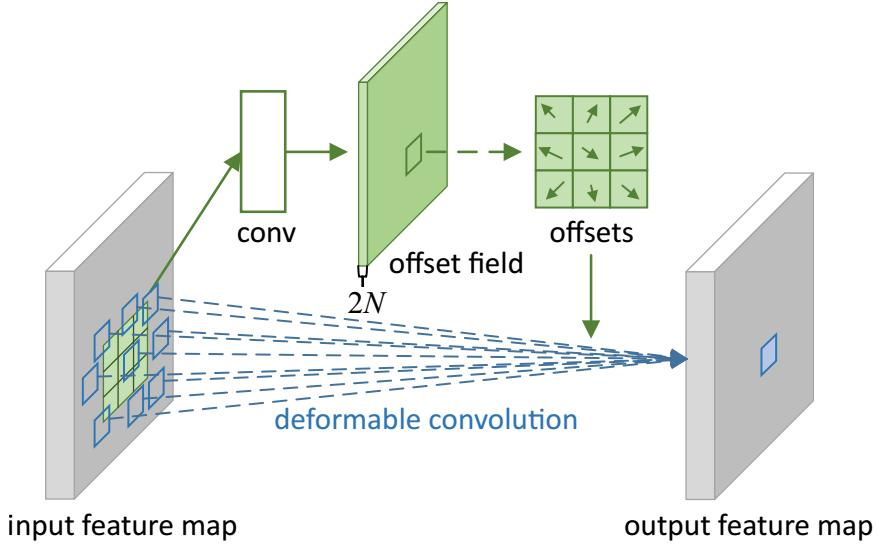
\includegraphics[height=6.5cm]{../graphic/dfconv.jpg}
            \end{figure}
            其中,$2N=2*k*k$, $k$表示卷积核的大小。
        \end{frame}

        \begin{frame}
            \frametitle{可变形卷积计算}
            将普通卷积分为两个步骤 \\
            1.规则采样:
            $$\mathcal{R}=\{(-1,-1),(-1,0),...,(0,1),(1,1)\}$$
            2.与卷积系数相乘并求和:
            $$y(p_0)=\sum_{p_n\in \mathcal{R}}w(p_n)\cdot x(p_0+p_n)$$
            其中,$p_0$是卷积中心。 \\
            \vspace{0.4cm}
            对于可变形卷积
            $$y(p_0)=\sum_{p_n\in \mathcal{R}}w(p_n)\cdot x(p_0+p_n+\Delta p_n)$$
            其中,$\Delta p_n$通过卷积计算得到。
        \end{frame}

        \begin{frame}
            \frametitle{可变形卷积效果图}
            \begin{figure}
                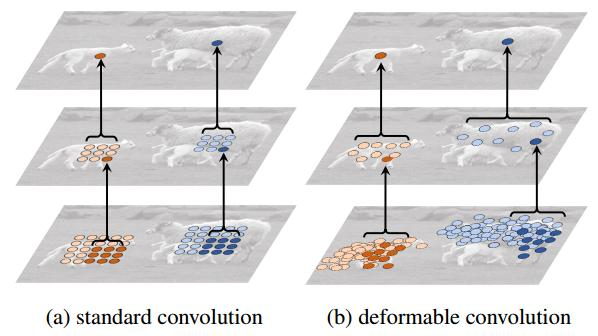
\includegraphics[height=6cm]{../graphic/dfconvvalid.jpg}
            \end{figure}
        \end{frame}

        \section{Focal Loss for Dense Object Detection 2017}
        \begin{frame}
            \frametitle{Focal Loss}
            对于二分类任务,交叉熵损失(Cross Entropy loss):
            $$\text{CE}(p)=-y\log(p)-(1-y)\log(1-p)$$
            $y$是样本标签为$1$或$0$,$p$是模型输出的判别概率。 \\
            \vspace{0.4cm}
            定义$p_t$
            $$p_t=\begin{cases} p &\text{if } y=1, \\ 1-p &\text{otherwise}\end{cases}$$
            那么
            $$\text{CE}(p_t)=-\log(p_t)$$
            定义Focal Loss
            $$\text{FL}(p_t)=-(1-p_t)^\gamma \log(p_t)$$
        \end{frame}
        
        \begin{frame}
            \frametitle{Focal Loss}
            \begin{figure}
                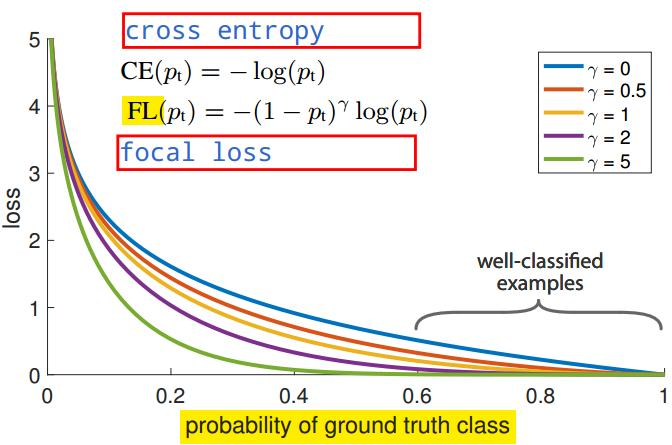
\includegraphics[height=6cm]{../graphic/focalloss.jpg}
            \end{figure}
        \end{frame}

        \begin{frame}
            \frametitle{目标检测框架}
            % \setbeamersize{}
            % \centering
            \begin{figure}
                \hspace*{-1.1cm}
                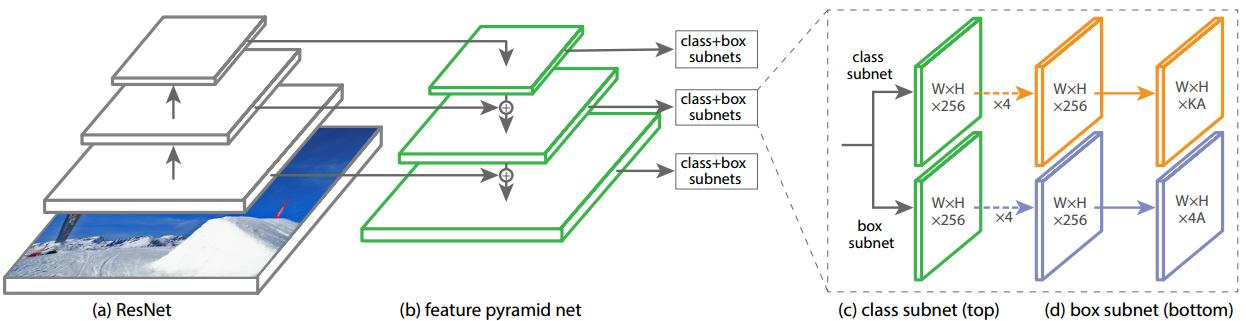
\includegraphics[height=3.3cm]{../graphic/retinanet.jpg}
            \end{figure}
            \vspace{0.2cm}
            $\oplus$表示element-wise add \\
            \vspace{0.3cm}
            $\times 4$表示同样的操作执行$4$次
         \end{frame}

         \begin{frame}
            % \frametitle{dfFaceNet}
            \begin{figure}
                \hspace*{-0.8cm}
                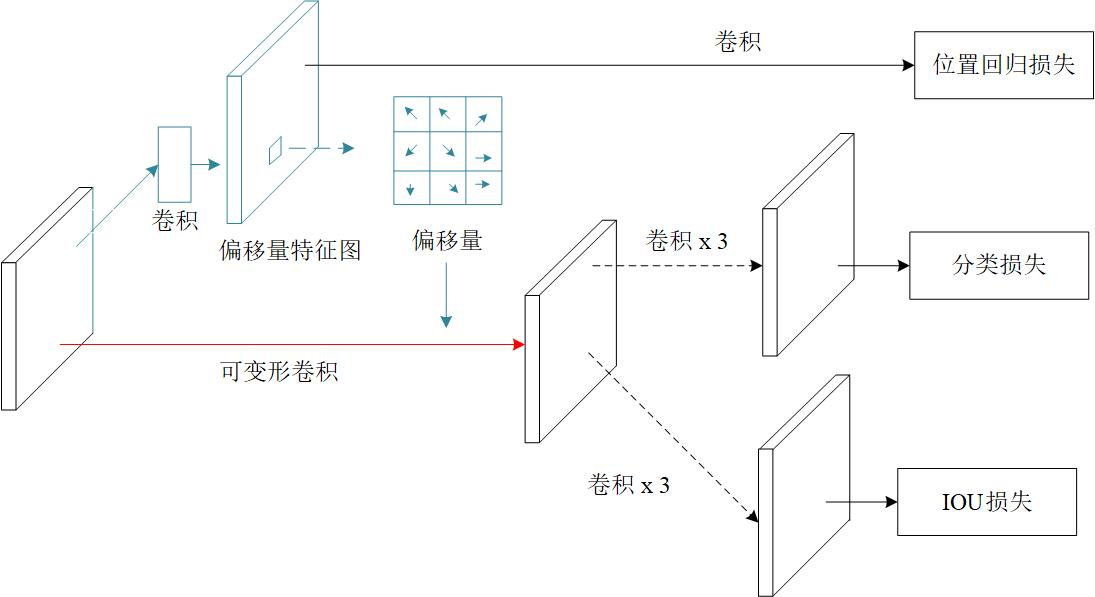
\includegraphics[height=6.6cm]{../graphic/dfFace2.jpg}
            \end{figure}
         \end{frame}
    \end{document}